 \documentclass[book.tex]{subfiles}
\begin{document}
\pagebreak

\section{Random Tricks}
Various smart techniques were employed to ensure every CPU cycle counted. This section describes random tricks used to increase game speed.


\subsection{Bouncing Physics}
When Keen throws a flower, it bounces off walls. For flat walls and floors, the bounce is easily calculated by reversing either the x-speed (for vertical walls) or the y-speed (for horizontal walls). However, handling bounces on slopes is more complex. Accurately calculating a bounce on a slope would require computationally expensive \cw{cos} and \cw{sin} operations.\\

\par
To simplify this, the game uses an algorithm that approximates the angle to one of four  values: 22$^{\circ}$, 45$^{\circ}$, 67$^{\circ}$ or 90$^{\circ}$. Based on the ratio between the x-speed and y-speed, the corresponding angle and speed is calculated. The angle values 0-3 refer to a positive \cw{xspeed}, and the values 4-7 to a negative \cw{xspeed}.\\

\par
\begin{figure}[H]
\centering
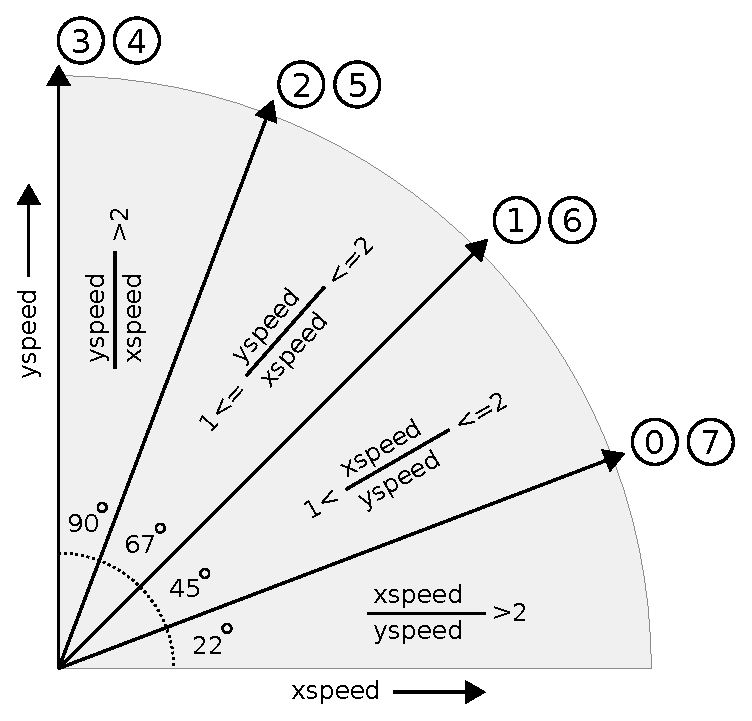
\includegraphics[width=0.8\textwidth]{imgs/drawings/angle_ratio.eps}
\label{fig:angles}
\end{figure}

\par
The resulting speed is determined as a factor of either the \cw{xspeed} or \cw{yspeed}, depending on which of the two has the larger absolute value. For higher precision, the speed is expressed in global coordinates and therefore multiplied by 256.\\

\par
\begin{minipage}{\textwidth}
  \lstinputlisting[language=C]{code/calc_angle.c}
\end{minipage}

\par
For each combination of the eight slope types and incoming angle, the bounce angle is determined using a simple lookup table. \\

\begin{figure}[H]
\centering
\setlength{\tabcolsep}{2pt} % set border margin to 3
\renewcommand{\arraystretch}{1.2}
\small
\begin{tabular}{
      >{\centering}p{0.18\textwidth}
      >{\centering}p{0.09\textwidth}|
      >{\centering}p{0.09\textwidth}|
      >{\centering}p{0.09\textwidth}|
      >{\centering}p{0.09\textwidth}|
      >{\centering}p{0.09\textwidth}|
      >{\centering}p{0.09\textwidth}|
      >{\centering}p{0.09\textwidth}|
      >{\centering\arraybackslash}p{0.09\textwidth}
}

 & \multicolumn{8}{c}{\textbf{incoming angle}} \\ 
\textbf{Wall type} & \textbf{0} & \textbf{1} & \textbf{2} & \textbf{3} & \textbf{4} & \textbf{5} & \textbf{6} & \textbf{7} \\ \hline
\textbf{0} & 0 & 0 & 0 & 0 & 0 & 0 & 0 & 0 \\ \hline
\textbf{1} & 7 & 6 & 5 & 4 & 3 & 2 & 1 & 0 \\ \hline
\textbf{2} & 5 & 4 & 3 & 2 & 1 & 0 & 15 & 14 \\ \hline
\textbf{3} & 5 & 4 & 3 & 2 & 1 & 0 & 15 & 14 \\ \hline
\textbf{4} & 3 & 2 & 1 & 0 &15 &14 & 13 & 12 \\ \hline
\textbf{5} & 9 & 8 & 7 & 6 & 5 & 4 & 3 & 2 \\ \hline
\textbf{6} & 9 & 8 & 7 & 6 & 5 & 4 & 3 & 2 \\ \hline
\textbf{7} &11 &10 & 9 & 8 & 7 & 6 & 5 & 4 \\ \hline

\end{tabular}\\
\setlength{\tabcolsep}{6pt} % reset border margin
\caption{Bounce lookup table \cw{bounceangle[8][8]}.}
\end{figure}


\par
Each entry in the table corresponds to one of 16 possible bounce angles. For example, when a wall type 3 slope is hit with an incoming angle of 22$^{\circ}$ and postive \cw{xspeed}, the lookup table refers to bounce angle \#5. Each bounce angle is decomposed into a new \cw{xspeed} and \cw{yspeed}.\\


\par
\begin{figure}[H]
\centering
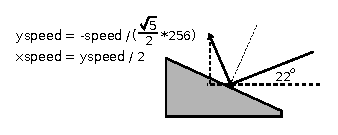
\includegraphics[width=0.7\textwidth]{imgs/drawings/bounce_angle.eps}
\caption{Wall type 3 with incoming angle of 22$^{\circ}$.}
\label{fig:bounce_angles}
\end{figure}
\par

\begin{minipage}{\textwidth}
  \lstinputlisting[language=C]{code/angle.c}
\end{minipage}

\bigskip
\par
It is worth noting that in some cases, the resulting bounce angle does not follow the laws of physics. For instance, an incoming angle of 22$^{\circ}$ on a 45$^{\circ}$ slope results in a bounce angle of 90$^{\circ}$ instead of the expected 67$^{\circ}$.\\

\par
\begin{figure}[H]
\centering

\includegraphics[width=0.4\textwidth]{imgs/drawings/bounce_physics.eps}
\caption{Incoming angle of 22$^{\circ}$ results in bounce angle of 90$^{\circ}$.}
\end{figure}
\par




\subsection{Screen fades}
When a new level is loaded, the screen fades from black to the default colors by reassigning the color palette. Each of the 16 color indices can be reprogrammed to any "RGBI" color, simply by calling the BIOS software interrupt \cw{10h}.\\

\par
\begin{minipage}{\textwidth}
  \lstinputlisting[language=C]{code/ega_set_palette.c}
\end{minipage}
\label{ega_set_palette}

\par
By using \cw{\_AX=1002h}, the entire palette can be reprogrammed at once. In this process, \cw{ES:BX} points to 17 bytes, where each byte represents an RGBI value for one of the 16 palette indices, plus one for the border.

\begin{figure}[H]
\centering
\setlength{\tabcolsep}{2pt} % set border margin to 2
\renewcommand{\arraystretch}{0.9}
\small
\begin{tabularx}{\textwidth}[c]{|+X|+X|+X|+X|+X|+X|+X|+X|+X|+X|+X|+X|+X|+X|+X|+X|+X|+X|}  
\hline

\rowcolor{CGA_White}\rowstyle{\color{black}}  \textbf{\#} & \textbf{0} & \textbf{1} & \textbf{2} & \textbf{3} & \textbf{4} & \textbf{5} & \textbf{6} & \textbf{7} & \textbf{8} & \textbf{9} & \textbf{10} & \textbf{11} & \textbf{12} & \textbf{13} & \textbf{14} & \textbf{15} & \textbf{16} \\ \hline

\rowcolor{CGA_Black}\rowstyle{\color{white}}   \cellcolor{CGA_White}\color{black} 0 &0& 0 & 0 & 0 & 0 & 0 & 0 & 0 & 0 & 0 & 0 & 0 & 0 & 0 & 0 & 0 & 0\\ \hline

\rowcolor{CGA_Black}\rowstyle{\color{white}}  \cellcolor{CGA_White}\color{black} 1 & 0 & 0 & 0 & 0 & 0 & 0 & 0 & 0 & 0 & \cellcolor{CGA_Blue} 1 & \cellcolor{CGA_Green}2 & \cellcolor{CGA_Cyan}3 & \cellcolor{CGA_Red}4 & \cellcolor{CGA_Magenta}5 & \cellcolor{CGA_Brown}6 & \cellcolor{CGA_Light_Grey}7  & 0\\ \hline

\rowcolor{CGA_Black}\rowstyle{\color{white}}  \cellcolor{CGA_White}\color{black} 2 & 0 & 0 & 0 & 0 & 0 & 0 & 0 & 0 & \cellcolor{CGA_Dark_Grey}0x18 & \cellcolor{CGA_Bright_Blue}0x19 & \cellcolor{CGA_Bright_Green}\color{black}0x1a & \cellcolor{CGA_Bright_Cyan}\color{black}0x1b & \cellcolor{CGA_Bright_Red}\color{black}0x1c & \cellcolor{CGA_Bright_Magenta}\color{black}0x1d & \cellcolor{CGA_Bright_Brown}\color{black}0x1e & \cellcolor{CGA_White}\color{black}0x1f & 0\\ \hline

\rowcolor{CGA_Black}\rowstyle{\color{white}}  \cellcolor{CGA_White}\color{black} 3 & 0 & \cellcolor{CGA_Blue} 1 & \cellcolor{CGA_Green}2 & \cellcolor{CGA_Cyan}3 & \cellcolor{CGA_Red}4 & \cellcolor{CGA_Magenta}5 & \cellcolor{CGA_Brown}6 & \cellcolor{CGA_Light_Grey}7 & \cellcolor{CGA_Dark_Grey}0x18 & \cellcolor{CGA_Bright_Blue}0x19 & \cellcolor{CGA_Bright_Green}\color{black}0x1a & \cellcolor{CGA_Bright_Cyan}\color{black}0x1b & \cellcolor{CGA_Bright_Red}\color{black}0x1c & \cellcolor{CGA_Bright_Magenta}\color{black}0x1d & \cellcolor{CGA_Bright_Brown}\color{black}0x1e & \cellcolor{CGA_White}\color{black}0x1f & 0\\ \hline

\rowcolor{CGA_White}\rowstyle{\color{white}}  \cellcolor{CGA_White}\color{black} 4 & \cellcolor{CGA_Black}0& \cellcolor{CGA_Blue} 1 & \cellcolor{CGA_Green}2 & \cellcolor{CGA_Cyan}3 & \cellcolor{CGA_Red}4 & \cellcolor{CGA_Magenta}5 & \cellcolor{CGA_Brown}6 & \cellcolor{CGA_Light_Grey}7 & \color{black}0x1f & \color{black}0x1f & \color{black}0x1f & \color{black}0x1f & \color{black}0x1f & \color{black}0x1f & \color{black}0x1f & \color{black}0x1f & \cellcolor{CGA_Black}0\\ \hline

\rowcolor{CGA_White}\rowstyle{\color{black}}  5&0x1f& 0x1f & 0x1f & 0x1f & 0x1f & 0x1f & 0x1f & 0x1f & 0x1f & 0x1f & 0x1f & 0x1f & 0x1f & 0x1f & 0x1f & 0x1f & 0x1f\\ \hline

\end{tabularx}\\
\setlength{\tabcolsep}{6pt} % reset border margin
\caption{Color fading table \cw{colors[7][17]}.}
\end{figure}

Fading the screen from black to color is straightforward.\\
\par
\begin{minipage}{\textwidth}
  \lstinputlisting[language=C]{code/ega_fade_in.c}
\end{minipage}
\label{ega_fade_in}


\end{document}



